\section{热力学过程的分析方法}
\subsection{状态关系、过程关系与能量关系}
一道热力学题通常需要三类方程。气态方程 $pV=nRT$ 联系同一平衡态的状态量；机械约束、传热条件或指定曲线确定过程关系；第一定律确定能量交换，取吸热与对外做功分别为正时，

\begin{equation}\label{eq:t3firstlaw}
 \Delta U=Q-W,\qquad Q=\Delta U+W.
\end{equation}
三类方程相互补充，任何一类通常都不能单独给出全部答案。式\eqref{eq:t3firstlaw}的符号约定应贯穿每一段过程与整个循环。

解题时先确定物质的量是否固定，再判断气体是否始终接近平衡。若有充气、放气或凝结，不能直接使用固定 $n$ 的关系；若有自由膨胀等强烈非平衡过程，初末态可以用状态方程，中间过程却不能任意画成一条气体状态曲线。

对于定量理想气体、恒定摩尔定容热容，端点总满足 $\Delta U=nC_V\Delta T=(C_V/R)\Delta(pV)$。因此先由端点求内能，再根据实际路径求功，最后由 $Q=\Delta U+W$ 求热量，是最稳定的计算顺序。

\subsection{准静态、可逆与绝热的区别}
准静态过程要求外界条件改变得足够缓慢，使系统能用一串接近平衡的状态描述。可逆过程还要求系统和环境能够共同沿原过程逆行，并恢复所有条件而不留下其他变化。慢过程若存在摩擦、有限温差传热等耗散，仍然不可逆。

绝热只表示指定边界没有热交换，即 $Q=0$。缓慢、无摩擦、无热交换的活塞运动可近似为可逆绝热；真空自由膨胀也可绝热，却显然不是准静态可逆过程。判定公式适用性时，这几个条件必须分别检查。

\fig{fig:h3:adiabaticmodels}{同为绝热，缓慢卸载的活塞膨胀有边界功，刚性容器向真空扩散没有边界功}{\begin{tikzpicture}

\draw[world](0,3)--(0,0)--(2,0)--(2,3);\fill[blue!8](0,0)rectangle(2,2);\draw[very thick](0,2)--(2,2);\draw[guide](0,1.2)--(2,1.2);\draw[guide,rounded corners](-.3,-.3)rectangle(2.3,3.1);\draw[world](.6,2)rectangle(1.4,2.4);\draw[flow](1,2.5)--(1,3.6)node[above]{逐渐卸载};\node at(1,-1){$Q=0,\quad W>0$};
\begin{scope}[xshift=5cm]\draw[world](0,0)rectangle(5,2.5);\draw[guide](2.5,0)--(2.5,2.5);\foreach \xx/\yy in {.5/.5,1.2/1.8,2.1/.8,3.2/1.7,4.2/.6}{\fill[blue](\xx,\yy)circle(.05);}\node at(2.5,3.3){隔板撤去后};\node at(2.5,-1){$Q=0,\quad W=0$};\end{scope}

\end{tikzpicture}}
图\ref{fig:h3:adiabaticmodels}左图通过微小地改变外负载，使活塞两侧接近机械平衡，才可在每一步用气体的$p\dd V$计算功。右图气体扩散到原来的真空区，容器外边界没有位移；即使气体所占空间增加，也没有同样的受力边界。二者都没有吸热，温度变化却不能用同一条绝热幂律判断。



此外，“绝热缸壁”只排除了通过缸壁的传热。若电阻通电、轴带动叶片或气体从入口流入，仍有其他形式的能量进入。题目的边界条件必须逐项转化为能量式中的相应项。

\section{等值过程与可逆绝热过程}
\subsection{等容与等压过程}
等容过程满足 $V=\text{常量}$、$p/T=\text{常量}$。若只存在体积功，则 $W=0$，$Q=nC_V\Delta T$。等容升温时吸热量等于内能增加；等容降温时放热，压强随温度下降。

等压过程满足 $p=\text{常量}$、$V/T=\text{常量}$。边界机械平衡时
\[W=p(V_f-V_i)=nR\Delta T,\qquad Q=nC_p\Delta T,\qquad C_p=C_V+R.
\]
第二讲已由膨胀功解释 $C_p-C_V=R$。本讲应用时，更要检查装置能否维持相应路径：活塞接触挡板后不再自由等压运动；例\ref{t3-3}的弹簧活塞压强随位置改变，也不能套用等压吸热公式。


若存在电功、搅拌功或流入物质，单凭体积不变不能推出吸热量等于内能增加。应先写完整能量关系，再使用状态函数求 $\Delta U$。条件“只存在体积功”是 $Q_V=nC_V\Delta T$ 的组成部分，不能在代公式时省去。

\subsection{等温与可逆绝热过程的比较}
定量理想气体等温时 $pV=nRT=\text{常量}$，内能不变。若过程可逆或准静态且无额外耗散，
\[W=nRT\int_{V_i}^{V_f}\frac{\dd V}{V}
=nRT\left[\ln\frac V{V_i}\right]_{V_i}^{V_f}
=nRT\ln\frac{V_f}{V_i},\qquad Q=W.
\]
膨胀时 $V_f>V_i$，$W,Q$ 均为正；压缩时二者均为负。对数函数的自变量必须是无量纲体积比，不能写成单独的 $\ln V$ 后忘记上下限。

等温并不意味着没有热传递。可逆等温膨胀中，气体持续对外做功，必须从热源吸收相等热量才能维持温度。等温压缩则把外界输入的功以热量形式排出。例\ref{t3-1}利用末段的等温压缩比较两条路径的热量。


对固定气体量，取 $C_V$ 为常量。绝热时 $\delta Q=0$，机械平衡给 $\delta W=p\dd V$，于是

\[nC_V\dd T=-p\dd V=-\frac{nRT}{V}\dd V.
\]
除以$nC_VT$，先把两个状态变量分离为$\dd T/T=-(R/C_V)\dd V/V$，再分别从初态积分到末态：
\[
\int_{T_i}^{T_f}\frac{\dd T}{T}
=-\frac R{C_V}\int_{V_i}^{V_f}\frac{\dd V}{V},\qquad
\left[\ln\frac T{T_i}\right]_{T_i}^{T_f}
=-\frac R{C_V}\left[\ln\frac V{V_i}\right]_{V_i}^{V_f}.
\]
代入上下限得到
\[\ln\frac{T_f}{T_i}=-\frac R{C_V}\ln\frac{V_f}{V_i}.
\]
由$R/C_V=\gamma-1$，对上式取指数，先得$T_f/T_i=(V_i/V_f)^{\gamma-1}$，整理为$T_fV_f^{\gamma-1}=T_iV_i^{\gamma-1}$。再将$T=pV/(nR)$代入，左、右两边分别成为$pV^\gamma/(nR)$，故$pV^\gamma$不变。若改用$V=nRT/p$消去体积，则$TV^{\gamma-1}=(nR)^{\gamma-1}T^\gamma p^{1-\gamma}$；固定气体量时前面的因子也是常量。因此得到三种等价形式
\[\boxed{TV^{\gamma-1}=\text{常量}},\qquad
\boxed{pV^\gamma=\text{常量}},\qquad
\boxed{T^\gamma p^{1-\gamma}=\text{常量}}.
\]
从推导中可以看出，每一项假设究竟用在何处：固定气体量使 $n$ 可从微分式中提出；绝热令 $\delta Q=0$；边界机械平衡使实际功可写成 $p\dd V$；恒定热容使积分成为对数之差。若其中一项改变，推导链就须相应调整，而不能只因题目出现“绝热”二字就跳到最终幂律。

气体对恒定外压突然膨胀时，实际功应由外压计算；入口充气时，分子数持续变化，$\dd U$也不再只是 $nC_V\dd T$。这两种情况分别失去了推导中的边界机械平衡条件与固定气体量条件，均须重新列能量方程。

功可由第一定律直接求得，
\[\boxed{W=nC_V(T_i-T_f)=\frac{p_iV_i-p_fV_f}{\gamma-1}}.
\]
可逆绝热膨胀通过消耗内能对外做功，温度下降；压缩时外界做功使温度上升。这与等温膨胀需要从热源补充热量形成鲜明的能量差别。

\fig{fig:iso-adia}{同一初态出发的等温与可逆绝热膨胀；图取$\gamma=7/5$}{\begin{tikzpicture}

\draw[axis](0,0)--(5,0)node[right]{$V$};\draw[axis](0,0)--(0,3.6)node[above]{$p$};\draw[flow,blue,domain=1:4,samples=100]plot(\x,{3/\x});\draw[flow,red,domain=1:4,samples=100]plot(\x,{3/(\x^1.4)});\fill(1,3)circle(.05)node[above]{$A$};\draw[guide](4,.75)--(4.5,1.1)node[right]{等温};\draw[guide](4,.430762)--(4.5,-.55)node[right]{绝热};\node at(3.3,2.7){$|\dd p/\dd V|_{\rm ad}=\gamma p/V$};

\end{tikzpicture}}

图\ref{fig:iso-adia}中，两曲线都从$A$出发，绝热线下降更快。对$pV=K_1$求微分，$V\dd p+p\dd V=0$给等温线斜率$\dd p/\dd V=-p/V$；对$pV^\gamma=K_\gamma$求微分，$V^\gamma\dd p+p\gamma V^{\gamma-1}\dd V=0$给绝热线斜率$\dd p/\dd V=-\gamma p/V$。在同一点，后者绝对值是前者的$\gamma$倍。比较曲线陡缓时必须从同一点、同一坐标尺度出发。

\subsection{自由膨胀与绝热压缩不可混同}
撤去气体与真空之间的隔板，若整个容器绝热刚性，外界不输入热量，真空也不提供边界阻力。因此 $Q=0,W=0,\Delta U=0$；理想气体达到新平衡后温度与初态相同。

这一步的始末温度相同，却不能把实际过程当作可逆等温过程求功。中间气体有流动、不均匀和耗散，无法用一条平衡双曲线描述。若误用等温可逆功，会算出并不存在的正功；若误用绝热幂律，则会算出并不存在的降温。

也可将自由膨胀和可逆等温膨胀放到同样的端点来比较。两者的理想气体温度相同、体积比相同，故内能差和熵差都相同；可逆等温膨胀却从热源吸热并对外做等量功，自由膨胀则两者都为零。相同的端点不能确定 $Q,W$，但可以确定 $\Delta U,\Delta S$。这种比较有助于区分“某条假想路径可用于算状态量”与“实际过程就按该路径发生”。

例\ref{t3-6}先自由膨胀，再可逆绝热压缩。两步分别使用不同物理条件；最终体积恢复，不代表温度、熵或外界做功也恢复。练习\ref{t3-13}进一步讨论为什么孤立气体不能自行逆转自由膨胀。

\subsection{用多方过程联系常见路径}
若给定过程满足 $pV^m=K$，且 $m$为常量，则称为多方过程。固定气体量、准静态且 $m\ne1$时，将 $p=KV^{-m}$代入功的积分，依次得到

\[
\begin{aligned}
 W&=K\int_{V_i}^{V_f}V^{-m}\,\dd V
 =K\left[\frac{V^{1-m}}{1-m}\right]_{V_i}^{V_f}\\
 &=\frac{K}{1-m}(V_f^{1-m}-V_i^{1-m})\\
 &=\frac{p_fV_f-p_iV_i}{1-m}
 =\frac{nR\Delta T}{1-m}.
\end{aligned}
\]
再将 $\Delta U=nC_V\Delta T$代入第一定律，才有
\[
 Q=n\left(C_V+\frac R{1-m}\right)\Delta T.
\]
积分方向已包含膨胀功为正、压缩功为负的区别。取 $m=0$恢复等压过程，$m=\gamma$时热量为零；$m=-1$则恢复第二讲 $p=kV$的结果。多方指数只描述指定路径，不自动保证过程可逆；题目没有给出路径时，不能自行假定 $m$。


括号内的量可视为沿该指定路径的摩尔过程热容，不是气体新的状态参数。它可能与 $C_V,C_p$ 不同，某些路径下甚至为负，表示气体温度升高时仍向外放热，由较大的外界压缩功提供内能增加。不能因此断言理想气体的定容热容为负。$m=1$ 时，路径由等温条件给定，应从 $W=nRT\ln(V_f/V_i)$ 重新计算。


\fig{fv:h3:paths}{经过同一初态的不同路径，具有不同斜率与曲线下面积}{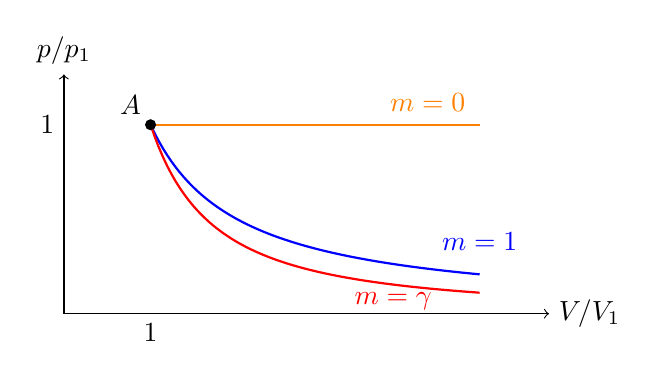
\begin{tikzpicture}[x=1.1cm,y=.8cm]
\draw[->](0,0)--(5.6,0)node[right]{$V/V_1$};\draw[->](0,0)--(0,3.8)node[above]{$p/p_1$};
\draw[blue,thick,domain=1:4.8,samples=80]plot(\x,{3/\x});\draw[red,thick,domain=1:4.8,samples=80]plot(\x,{3/pow(\x,1.4)});
\draw[orange,thick](1,3)--(4.8,3);\fill(1,3)circle(2pt)node[above left]{$A$};\node[left]at(0,3){$1$};\node[below]at(1,0){$1$};
\node[orange]at(4.2,3.35){$m=0$};\node[blue]at(4.8,1.15){$m=1$};\node[red]at(3.8,.2){$m=\gamma$};\end{tikzpicture}}
图\ref{fv:h3:paths}中的 $m$指多方指数，$pV^m=\text{常量}$给局部斜率 $\dd p/\dd V=-mp/V$。从同一状态膨胀，绝热线比等温线下降更快，因而到相同体积时温度更低、对外功也更小。路径方程只把状态变量联系起来；热量仍须由 $Q=\Delta U+\int p\dd V$另算。尤其 $m=1$的积分是对数，不能直接代入含 $1-m$分母的普通幂积分式。


\section{非标准装置与开口充气}
\subsection{由受力和几何求路径，再积分求功}
弹簧活塞平衡时，$pS=p_0S+kx$，体积为 $V=V_i+Sx$，所以
\[p=p_0+\frac{k}{S^2}(V-V_i).
\]
这是一条 $p$--$V$ 直线，功既可由梯形面积求出，也可分为 $p_0\Delta V+\frac12kx^2$。前一项是对大气做功，后一项是弹簧储能，两个计算应一致。随后再由 $\Delta U=(C_V/R)\Delta(pV)$ 求热量，而不是先选 $C_p\Delta T$。

\fig{fig:h3:springpath}{弹簧压缩随活塞位移增加；压力路径的斜率由$k/S^2$决定}{\begin{tikzpicture}

\draw[world](0,2)--(0,0)--(6,0) (0,2)--(6,2);\fill[blue!8](0,0)rectangle(3,2);\draw[very thick](3,0)--(3,2);\draw[guide](2,0)--(2,2);\draw[world](5.5,0)--(5.5,2);\draw[decorate,decoration={zigzag,segment length=3pt,amplitude=2pt}](3,1)--(5.5,1);\node at(1.3,1){气体};\draw[flow](2,2.6)--(3,2.6)node[midway,above]{$x$};\draw[force](3,.4)--(4.2,.4)node[right]{$pS$};\draw[force](4.2,1.6)--(3,1.6);\node at(4.7,2.65){$p_0S+kx$};\node at(3,-.8){$\Delta V=Sx,\quad W=p_0\Delta V+kx^2/2$};

\end{tikzpicture}}
图\ref{fig:h3:springpath}的虚线是弹簧无形变时的活塞位置。气体向右推动活塞，压强须同时克服大气和弹簧；弹簧越压缩，所需$p$越高。若初态已有预紧量$x_0$，受力式应改为$pS=p_0S+k(x_0+x)$，直线的截距也随之改变，不能只改体积而漏掉初始负载。



连通双缸中，气体内部可发生不可逆流动，但对整个封闭气体系统仍可使用第一定律。若唯一外边界是承受恒定外压的活塞，边界功可按该外压与实际位移求出。例\ref{t3-4}中，另一室原为真空，气体分布改变与外界压缩同时存在，因此温度变化须由整体能量守恒决定。


受力式中的弹簧伸长应相对自然长度量取，体积式中的位移则相对选定初态量取；两者若起点不同，必须保留初始预紧量。活塞自重或附加重物也应按方向列入力平衡，不能一律省入大气压而不说明。


一旦遇到挡板或弹簧失去接触，机械约束改变，压强与体积的路径也随之切换。应在切换点保留同一个物理状态，再分别计算前后两段功。若直接把原先的直线路径延伸到接触之后，即使代数积分正确，也已经计算了另一种装置过程。

\subsection{焓中的推动功从哪里来}
固定容器充气时，物质穿过边界，进入气体不仅携带内能。设进入 $\dd n$ mol气体，占入口体积 $\dd V_{\text{入}}$，上游气体还需做 $p\dd V_{\text{入}}=RT\dd n$ 的功把它推入容器。因此每摩尔进入的流动能量为

\[h=u+p\bar V=C_VT+RT=C_pT.
\]
$h$ 称为摩尔焓。它不是额外制造的能量，而是把流体内能和通过入口所伴随的推动功合并，便于列控制体能量关系。若入口速度或高度变化不可忽略，还要加上每摩尔动能与重力势能。

\fig{fig:flow-enthalpy}{入口微团受上游压力推动；内能和推动功随同一批物质进入刚性容器}{\begin{tikzpicture}

\draw[world](0,.8)--(4,.8) (0,1.7)--(4,1.7);\draw[world](4,.8)--(4,0)--(7,0)--(7,2.6)--(4,2.6)--(4,1.7);\draw[guide,rounded corners](3.8,-.2)rectangle(7.2,2.8);\fill[blue!12](2,.8)rectangle(3.1,1.7);\draw[very thick](2,.8)--(2,1.7);\draw[force](.7,1.25)--(2,1.25)node[midway,above]{$pS$};\node at(2.55,1.25){$\dd n$};\draw[flow](3.1,1.25)--(4.7,1.25);\node at(5.7,1.3){容器内能$U$};\draw[dim](2,.3)--(3.1,.3)node[midway,below]{$\dd\ell$};\node at(3.5,-1.2){$pS\dd\ell=p\dd V_{\text{入}}=RT\dd n$};

\end{tikzpicture}}

图\ref{fig:flow-enthalpy}把推动功画在控制体之外，避免与容器内气体的体积功混淆。刚性容器的外壁不动，所以没有外壁体积功；入口仍可把焓随物质带入，二者并不矛盾。


当壁热容、入口动能与势能、热交换及轴功都可忽略时，固定控制体满足
\[U_f-U_i=\int_0^{n_f-n_i}h_{\text{入}}\,\dd n_{\text{入}}.
\]
若上游气库温度恒为 $T_s$，理想气体热容恒定，则
\[n_fC_VT_f-n_iC_VT_i
=C_pT_s[n_{\text{入}}]_0^{n_f-n_i}
=(n_f-n_i)C_pT_s.
\]
还需结合容器状态方程及停止充气的条件，例如末压等于气库压强。没有第二个状态条件，仅靠能量式不能同时确定 $n_f,T_f$。

列充气方程时，进入量是 $n_f-n_i$，不能把末气体量 $n_f$ 全部当作新流入的气体。容器原有分子也会被加热，但它们没有再次通过入口，所以只出现在内能端点中。另一方面，气库温度恒定控制的是每摩尔流入焓，不直接控制接收容器温度。把“气库恒温”误读成“容器始终等温”，会使能量式和末压条件相互矛盾。

对于初始真空的容器，$n_i=0$，直接得到 $T_f=(C_p/C_V)T_s$。容器内温度可以高于气库温度，因为进入的气体接受了上游推动功。若随后允许与环境传热，冷却到环境温度是另一个过程。例\ref{t3-5}和练习\ref{t3-11}分别处理非真空和真空初态。

\section{循环、热机与制冷机}
\subsection{逐段确定吸热量与放热量}
热机经过一周后回到初态，净内能变化为零。记所有吸热段热量之和为 $Q_h>0$，所有放热段热量绝对值之和为 $Q_c>0$，则

\[W_{\text{净}}=Q_h-Q_c,\qquad\boxed{\eta=\frac{W_{\text{净}}}{Q_h}=1-\frac{Q_c}{Q_h}}.
\]
如果某一段的热量符号不明显，可把过程分成微元，检查 $\delta Q=nC_V\dd T+p\dd V$ 的符号。两项同号时可直接判断；两项异号时必须比较大小。这一步对曲线路径尤其重要，因为整段可能跨过吸放热分界。只有证明一段始终吸热，才可将它的代数热量全部放入 $Q_h$。同样，循环中两个放热段的绝对值要相加，而不是把它们再与吸热相抵后作效率分母。

膨胀、压缩是机械分类，吸热、放热是能量交换分类，不能互相替代。例如可逆绝热膨胀有正功却不吸热；压缩过程中若内能增量足够大，也可能需要吸热。$p$--$V$ 循环面积只给净功，不直接给 $Q_h$。

例\ref{t3-8}中只有两条等压段交换热量，绝热线联系两段温度比；例\ref{t3-9}中应先证明只有斜直线段吸热，才能用三角形面积除以相应吸热量。循环面积同比放大时，效率未必改变。


逆向运行需要外界输入功 $W_{\text{入}}=Q_h-Q_c$。制冷机关注从低温端取走的热量，热泵关注向高温端送出的热量，因而定义

\[\varepsilon=\frac{Q_c}{W_{\text{入}}},\qquad\mathrm{COP}_h=\frac{Q_h}{W_{\text{入}}}=\varepsilon+1.
\]
这两个系数不是热机效率，可以大于1。高温端得到的热量由输入功与从低温端搬运的热量共同组成；不能据系数大于1判断违反能量守恒。

\fig{fig:engine-flow}{热机与制冷机的热量和功的方向}{\begin{tikzpicture}[x=1cm,y=1cm]
\draw[world] (0,3) rectangle (2,3.8) (0,1.2) rectangle (2,2.2) (0,-.5) rectangle (2,.3);\node at (1,3.4){高温源};\node at (1,1.7){热机};\node at (1,-.1){低温源};\draw[flow] (1,3)--(1,2.2) node[midway,right]{$Q_h$};\draw[flow] (1,1.2)--(1,.3) node[midway,right]{$Q_c$};\draw[flow] (2,1.7)--(3.5,1.7) node[right]{$W$};\draw[world] (6,3) rectangle (8,3.8) (6,1.2) rectangle (8,2.2) (6,-.5) rectangle (8,.3);\node at (7,3.4){高温源};\node at (7,1.7){制冷机};\node at (7,-.1){低温源};\draw[flow] (7,2.2)--(7,3) node[midway,right]{$Q_h$};\draw[flow] (7,.3)--(7,1.2) node[midway,right]{$Q_c$};\draw[flow] (4.5,1.7)--(6,1.7) node[midway,above]{$W_{\text{入}}$};
\end{tikzpicture}}

图\ref{fig:engine-flow}应与循环方向一起读。无论机器怎样运行，能量守恒都成立；区别在于哪个方向的功是输入、哪个热量是目标。练习\ref{t3-12}据此计算卡诺制冷与热泵系数。

\section{第二定律、卡诺循环与熵判据}
\subsection{第二定律限制什么}
能量守恒只限制能量数量，不单独决定过程方向。两个不同温度物体接触时，热量自发由高温端流向低温端；反向传热若要持续发生，须有外界做功等其他变化。第一定律并不禁止反向传热，第二定律才给出方向约束。

常用表述有两种：不能制造一种循环装置，只从单一热源吸热并全部变成功而不产生其他变化；不能使热量只从低温物体传向高温物体而不产生其他变化。必须审查完整循环和环境，不能把一次非循环的等温膨胀误判为第二类永动机。

两种表述等价。若有单热源全转功的循环机，便可用其功驱动普通制冷机，组合后只留下热从低温端流向高温端；若有不需功的反向传热机，便可与普通热机组合，消除其向冷源排热的影响，得到单热源全转功装置。

\subsection{卡诺循环的四个过程与效率}
卡诺循环由高温 $T_h$ 下等温膨胀、可逆绝热膨胀、低温 $T_c$ 下等温压缩、可逆绝热压缩组成。两条等温段与热源交换热量，两条绝热段改变温度而不交换热量。

\fig{fig:carnot}{卡诺循环的四条实际可逆路径；图取$\gamma=5/3,T_c/T_h=1/2$示意}{\begin{tikzpicture}

\draw[axis](0,0)--(7,0)node[right]{$V$};\draw[axis](0,0)--(0,3.7)node[above]{$p$};
\draw[flow,red,domain=1:2,samples=90]plot(\x,{3/\x});\draw[flow,domain=2:5.656854,samples=100]plot(\x,{1.5*(2/\x)^(5/3)});\draw[flow,blue,domain=5.656854:2.828427,samples=100]plot(\x,{1.5/\x});\draw[flow,domain=2.828427:1,samples=100]plot(\x,{3/\x^(5/3)});
\node[above left]at(1,3){$A$};\node[above right]at(2,1.5){$B$};\node[above right]at(5.656854,.265165){$C$};\node[below left]at(2.828427,.53033){$D$};\node[red]at(1.7,2.5){$T_h$};\node[blue]at(4,.9){$T_c$};

\end{tikzpicture}}

图\ref{fig:carnot}中，$Q_h=nRT_h\ln(V_B/V_A)$，$Q_c=nRT_c\ln(V_C/V_D)$。两条绝热线分别给 $T_hV_B^{\gamma-1}=T_cV_C^{\gamma-1}$ 和 $T_hV_A^{\gamma-1}=T_cV_D^{\gamma-1}$，相除得 $V_B/V_A=V_C/V_D$。因此

\[\boxed{\eta_C=1-\frac{T_c}{T_h}}.
\]
温度必须用K，且该结论要求机器只与这两个恒温热源交换热量。实际热源温度变化或存在其他热交换时，不能把某两个端点温度直接代入卡诺效率。

一般循环中气体的最高、最低温度不能代替两个恒温热源温度。例如两等压两绝热循环在等压段连续变温换热，须先由绝热线建立成对温度比，再比较等压段温差；例\ref{t3-8}将据此求效率。

若某热机效率比同两热源间的可逆机更高，可令其驱动逆向可逆机，并调节循环次数使两者功相抵。组合后将只剩从低温源向高温源的净传热，违反第二定律，故任何热机效率不超过可逆机。同两热源间所有可逆机的效率也必须相同。

\subsection{理想气体的熵差及使用范围}
熵是状态量。为求两个平衡态的熵差，可沿任意连接它们的假想可逆路径积分，即使实际过程不可逆。定量理想气体热容恒定时，

\[\dd S=\frac{\delta Q_{\text{可逆}}}T=\frac{nC_V\dd T+p\dd V}{T},
\]
用理想气体状态方程$p/T=nR/V$，将温度项与体积项分开，再按图中路径分别积分。
\fig{fig:h3:entropyroute}{连接相同端点的假想可逆路径：先等容调温，再等温改变体积}{\begin{tikzpicture}

\draw[axis](0,0)--(5,0)node[right]{$V$};\draw[axis](0,0)--(0,3.8)node[above]{$T$};\draw[flow,blue](1,1)--(1,3);\draw[flow,red](1,3)--(4,3);\fill(1,1)circle(.05)node[left]{$A$};\fill(1,3)circle(.05)node[above left]{$B$};\fill(4,3)circle(.05)node[above right]{$C$};\draw[guide](0,1)--(1,1) (0,3)--(1,3) (1,0)--(1,1) (4,0)--(4,3);\node[left]at(0,1){$T_i$};\node[left]at(0,3){$T_f$};\node[below]at(1,0){$V_i$};\node[below]at(4,0){$V_f$};\node[blue,right]at(1.15,1.8){$V=V_i$};\node[red]at(2.7,3.6){$T=T_f$};

\end{tikzpicture}}
图\ref{fig:h3:entropyroute}中，$AB$保持体积不变，$BC$保持末温$T_f$不变。应把两段分别按其变量与端点积分：
\[
\Delta S_{AB}=nC_V\int_{T_i}^{T_f}\frac{\dd T}{T}
=nC_V\left[\ln\frac T{T_i}\right]_{T_i}^{T_f}
=nC_V\ln\frac{T_f}{T_i},
\]
\[
\Delta S_{BC}=nR\int_{V_i}^{V_f}\frac{\dd V}{V}
=nR\left[\ln\frac V{V_i}\right]_{V_i}^{V_f}
=nR\ln\frac{V_f}{V_i}.
\]
相加得到
\[
\boxed{\Delta S=nC_V\ln\frac{T_f}{T_i}+nR\ln\frac{V_f}{V_i}}.
\]实际过程只要有相同的初末平衡态，熵差便相同；图上的两段是计算状态量所选的可逆途径，不能据此把真实过程的功或热量也改成这两段的值。



对一段温度改变的实际过程，一般不能写 $\Delta S=Q/T$：热量可能在不同温度下交换，过程也可能不可逆。熵差公式的推导可以选“先等容改变温度、再等温改变体积”的假想可逆路径，两段分别给出对数项。由于熵是状态量，这个结果才可用于真实不可逆过程。恒温热源的温度始终不变，其熵变则可直接写成失去热量除以热源温度的负值。

可逆绝热过程 $\Delta S=0$；理想气体绝热自由膨胀的始末温度相同，而体积增加，故 $\Delta S=nR\ln(V_f/V_i)>0$。这个结果同时说明“绝热”不等于“熵不变”。

\fig{fig:h3:carnotTS}{卡诺循环在$T$--$S$图中为矩形，等温段的面积给热量，竖直段为等熵过程}{\begin{tikzpicture}

\draw[axis](0,0)--(5,0)node[right]{$S$};\draw[axis](0,0)--(0,3.8)node[above]{$T$};\fill[red!8](1,0)rectangle(4,3);\fill[white](1,0)rectangle(4,1.3);\draw[flow,red](1,3)--(4,3);\draw[flow](4,3)--(4,1.3);\draw[flow,blue](4,1.3)--(1,1.3);\draw[flow](1,1.3)--(1,3);\node[above left]at(1,3){$A$};\node[above right]at(4,3){$B$};\node[below right]at(4,1.3){$C$};\node[below left]at(1,1.3){$D$};\node[left]at(0,3){$T_h$};\node[left]at(0,1.3){$T_c$};\draw[dim](1,-.7)--(4,-.7)node[midway,below]{$\Delta S$};\node at(2.5,2.1){$W=(T_h-T_c)\Delta S$};

\end{tikzpicture}}
图\ref{fig:h3:carnotTS}用熵坐标重画同一循环。沿可逆路径有$\delta Q=T\dd S$，高、低温等温段的热量大小分别为$T_h\Delta S$与$T_c\Delta S$；两绝热段保持$S$不变。相同的水平宽度解释了热量比为何只等于温度比，矩形面积则对应净功。这里的几何面积表示热量，是因为纵轴为$T$、横轴为$S$，不能与任意坐标图的面积混用。




若系统从恒温热源吸热 $Q$，热源熵变为 $-Q/T_{\text{源}}$。这里 $Q$ 以系统吸热为正；热源若吸热，则 $Q<0$。必须先画清整体边界，再使用熵不减判据。图\ref{fig:entropy-boundary}把气体与唯一参与换热的热源一起包入虚线边界，外部不再有热量、物质或功的交换，因而这个整体是孤立系统，有

\[
 \boxed{\Delta S_{\text{总}}
 =\Delta S_{\text{气体}}-\frac Q{T_{\text{源}}}\ge0}.
\]
\fig{fig:entropy-boundary}{箭头规定气体吸热的正向；气体与参与换热的热源共同构成孤立整体}{\begin{tikzpicture}

\draw[guide,rounded corners](-.6,-1.6)rectangle(8.6,1.8);\node[above]at(4,1.8){孤立整体边界};\node[draw,minimum width=2.5cm,minimum height=1.4cm,align=center](R)at(1,0){恒温热源\\$T_{\text{源}}$};\node[draw,minimum width=2.8cm,minimum height=1.4cm,align=center](G)at(6.6,0){气体\\$\Delta S_{\text{气体}}$};\draw[flow](R.east)--(G.west)node[midway,above]{$Q$（吸热为正）};\node[below]at(1,-.9){$\Delta S_{\text{源}}=-Q/T_{\text{源}}$};\node[below]at(6.6,-.9){$\Delta S_{\text{气体}}$可正可负};

\end{tikzpicture}}
图\ref{fig:entropy-boundary}的箭头规定$Q$的正向。$Q>0$时，熵不等式要求$\Delta S_{\text{气体}}\ge Q/T_{\text{源}}>0$；若气体放热，则$Q<0$，气体本身可以减熵，但必须由热源增熵补偿。因此给定传热方向后，气体熵变的符号也受到约束。


闭口系统只保证没有物质穿过边界，仍可能向外放热而减熵，因此不能把“闭口”或“封闭”直接等同于“孤立”。若还涉及其他热源、物体或质量流动，就要继续扩大边界或分别计入相应熵变，不能只把气体与某一个热源相加便宣称整体熵不减。对于图示的孤立整体，可逆过程取等号，存在不可逆性时总熵增加。


最简单的方向检验是两个恒温热源间传热：若热量 $Q>0$ 从 $T_h$ 流向 $T_c<T_h$，则

\[
 \Delta S_{\text{总}}=-\frac Q{T_h}+\frac Q{T_c}
 =Q\left(\frac1{T_c}-\frac1{T_h}\right)>0.
\]
将同一传热方向反转，就会得到负值，说明它不能在没有其他变化的条件下自发发生。能量守恒只要求流出与流入的热量相等，熵判据才进一步限制方向。总熵非负是过程可行的必要条件；某个设想通过这一检验后，仍须满足装置约束和其他守恒关系。

例\ref{t3-7}给出的末态可形式上满足受力、气态方程与能量守恒，却导致总熵减少。因此该题的关键不只是算出热量，而是检验末态、热源和过程约束是否相容。仅凭某一步不满足泊松关系不能排除不可逆过程，总熵判据才提供了更一般的必要条件。


对固定 $n,\gamma$ 的同种理想气体，可逆绝热线满足 $pV^\gamma=K$。若两条曲线在同一点相交，该点给出的 $K$ 相同，两条曲线就是同一条线；因此不同可逆绝热线不相交。用熵作标记时，也可理解为不同等熵线不相交。

第一类永动机违反能量守恒；第二类永动机即使形式上不违反能量守恒，仍违反第二定律。持续输出功的装置必须交代能量从哪里转入、哪些物体或环境发生变化；判断循环时尤其要确认装置确已回到初态，而不是消耗了某种未列出的储能。

